\documentclass[12pt,letterpaper]{article}
\usepackage{graphicx,textcomp}
\usepackage{natbib}
\usepackage{setspace}
\usepackage{fullpage}
\usepackage{color}
\usepackage[reqno]{amsmath}
\usepackage{amsthm}
\usepackage{fancyvrb}
\usepackage{amssymb,enumerate}
\usepackage[all]{xy}
\usepackage{endnotes}
\usepackage{lscape}
\newtheorem{com}{Comment}
\usepackage{float}
\usepackage{hyperref}
\newtheorem{lem} {Lemma}
\newtheorem{prop}{Proposition}
\newtheorem{thm}{Theorem}
\newtheorem{defn}{Definition}
\newtheorem{cor}{Corollary}
\newtheorem{obs}{Observation}
\usepackage[compact]{titlesec}
\usepackage{dcolumn}
\usepackage{tikz}
\usetikzlibrary{arrows}
\usepackage{multirow}
\usepackage{xcolor}
\newcolumntype{.}{D{.}{.}{-1}}
\newcolumntype{d}[1]{D{.}{.}{#1}}
\definecolor{light-gray}{gray}{0.65}
\usepackage{url}
\usepackage{listings}
\usepackage{color}
\usepackage{graphicx}

\definecolor{codegreen}{rgb}{0,0.6,0}
\definecolor{codegray}{rgb}{0.5,0.5,0.5}
\definecolor{codepurple}{rgb}{0.58,0,0.82}
\definecolor{backcolour}{rgb}{0.95,0.95,0.92}

\lstdefinestyle{mystyle}{
	backgroundcolor=\color{backcolour},   
	commentstyle=\color{codegreen},
	keywordstyle=\color{magenta},
	numberstyle=\tiny\color{codegray},
	stringstyle=\color{codepurple},
	basicstyle=\footnotesize,
	breakatwhitespace=false,         
	breaklines=true,                 
	captionpos=b,                    
	keepspaces=true,                 
	numbers=left,                    
	numbersep=5pt,                  
	showspaces=false,                
	showstringspaces=false,
	showtabs=false,                  
	tabsize=2
}
\lstset{style=mystyle}
\newcommand{\Sref}[1]{Section~\ref{#1}}
\newtheorem{hyp}{Hypothesis}

\title{Problem Set 4}
\date{Due: April 12, 2024}
\author{Applied Stats II}


\begin{document}
	\maketitle
	\section*{Instructions}
	\begin{itemize}
	\item Please show your work! You may lose points by simply writing in the answer. If the problem requires you to execute commands in \texttt{R}, please include the code you used to get your answers. Please also include the \texttt{.R} file that contains your code. If you are not sure if work needs to be shown for a particular problem, please ask.
	\item Your homework should be submitted electronically on GitHub in \texttt{.pdf} form.
	\item This problem set is due before 23:59 on Friday April 12, 2024. No late assignments will be accepted.

	\end{itemize}

	\vspace{.25cm}
\section*{Question 1}
\vspace{.25cm}
\noindent We're interested in modeling the historical causes of child mortality. We have data from 26855 children born in Skellefteå, Sweden from 1850 to 1884. Using the "child" dataset in the \texttt{eha} library, fit a Cox Proportional Hazard model using mother's age and infant's gender as covariates. Present and interpret the output.

 \lstinputlisting[language=R, firstline=1,lastline=22]{PS4_answers_Jie.R}
 % Table created by stargazer v.5.2.3 by Marek Hlavac, Social Policy Institute. E-mail: marek.hlavac at gmail.com
 % Date and time: 周四, 4月 11, 2024 - 14:35:25
\begin{figure}[ht]
	\centering
	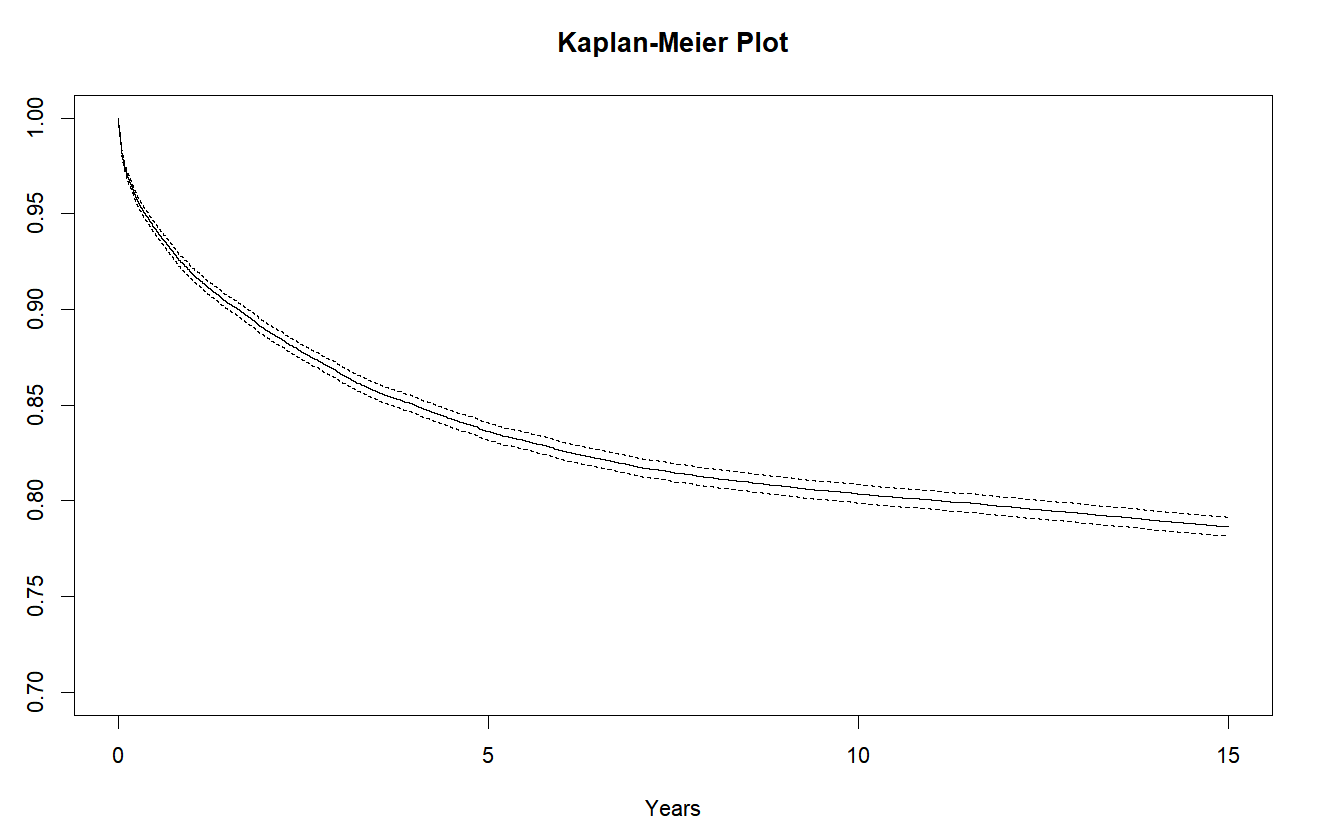
\includegraphics[width=1\textwidth]{picture1.png}  
\end{figure}
According to the picture, the survival rate decreases fastest from 0 to 5 years from 1 to about 0.8, which means that the survival risk is high during this period; the curve decreases slowly from 5 to 15 years, which means that the survival risk is low during this period.
\pagebreak
 \begin{table}[!htbp] \centering 
 	\caption{} 
 	\label{} 
 	\begin{tabular}{@{\extracolsep{5pt}}lc} 
 		\\[-1.8ex]\hline 
 		\hline \\[-1.8ex] 
 		& \multicolumn{1}{c}{\textit{Dependent variable:}} \\ 
 		\cline{2-2} 
 		\\[-1.8ex] & child\_surv \\ 
 		\hline \\[-1.8ex] 
 		m.age & 0.008$^{***}$ \\ 
 		& (0.002) \\ 
 		& \\ 
 		sexfemale & $-$0.082$^{***}$ \\ 
 		& (0.027) \\ 
 		& \\ 
 		\hline \\[-1.8ex] 
 		Observations & 26,574 \\ 
 		R$^{2}$ & 0.001 \\ 
 		Max. Possible R$^{2}$ & 0.986 \\ 
 		Log Likelihood & $-$56,503.480 \\ 
 		Wald Test & 22.520$^{***}$ (df = 2) \\ 
 		LR Test & 22.518$^{***}$ (df = 2) \\ 
 		Score (Logrank) Test & 22.530$^{***}$ (df = 2) \\ 
 		\hline 
 		\hline \\[-1.8ex] 
 		\textit{Note:}  & \multicolumn{1}{r}{$^{*}$p$<$0.1; $^{**}$p$<$0.05; $^{***}$p$<$0.01} \\ 
 	\end{tabular} 
 \end{table} \\
 The coefficient of m.age is 0.007617, which means that for every unit increase in maternal age, the hazard ratio increases by 1.007646 times, and the p-value of the coefficient is less than and not equal to 0.01, so the coefficient is statistically significant.\vspace{.25cm}\\
 The coefficient of sexfemale is -0.082215, which means that compared with the reference group, the risk ratio of women is reduced to 0.921074 times, and the p-value of the coefficient is less than and not equal to 0.01, so the coefficient is statistically significant.
 
\end{document}
